\documentclass{supervision}
\usepackage{course}

\Supervision{6}
\begin{document}
  \begin{questions}
    %%%%%%%%%%%%%%%%%%%%%%%%%%%%%%%%%%%%%%%%%%
    \section*{Topic 06 - Network Applications}
    %%%%%%%%%%%%%%%%%%%%%%%%%%%%%%%%%%%%%%%%%%
    \SetQuestionNumber{22}
    \question Internet Applications
    \begin{parts}
      \part HTTP is an application protocol, built on TCP, which was originally
        designed to allow retrieval of hypertext documents. Firewalls are
        application-level gateways (or routers) which aim to filter out
        malicious, illegal or unauthorised IP traffic based on the contents of
        packet payloads.
        \begin{subparts}
          \subpart Explain why network firewalls traditionally accept inbound
            HTTP traffic, but may not accept traffic for other services such as
            network filesystems or e-mail transfer (SMTP).
            \begin{solution}
              Web servers are very common and almost always designed to be
              accessible to the internet, where as access to networked file
              systems should be restricted to the local network.
            \end{solution}

          \subpart Describe the similarities and differences between an
            e-mail gateway (as might have been found joining two wide-area
            networks before the advent of IP) and an application-level
            firewall.
            \begin{solution}
              They are similar in that they form the boundary between two
              networks and can control what travels across the boundary but are
              different since one is concerned with the security of a network
              and the other is not.
            \end{solution}

          \subpart In modern networks, HTTP is used as a transport for remote
            procedure call, e-mail and even networked filesystems. A network
            engineer proposes that, to counter security concerns regarding some
            types of HTTP traffic, there is a need for a higher-level firewall
            which can selectively filter these. Suggest why this is more
            difficult than a firewall operating at the levels of TCP and UDP,
            and explain why this does not solve the security problem.
            \begin{solution}
              This is much more difficult as the firewall would have to parse
              and analyse the entire HTTP request which may be split across
              many packets and thus it would have to hold the packets until it
              could identify what they were.

              It would always be possible to tunnel any disallowed protocol
              over an allowed one.
            \end{solution}

        \end{subparts}
      \part Consider a case where a client $A$ is retrieving files $F$ and $G$
        from web site $B$. $F$ and $G$ are both \SI{125}{KB} (i.e., one
        megabit).
        \begin{subparts}
          \subpart The RTT between $A$ and $B$ is \SI{10}{ms} (note, these are
            roundtrip-times, not one-way latencies), and the bandwidth between
            the sites is \SI{10}{Mbps}. Assume all TCP SYN/ACK packets and HTTP
            request packets are negligible in size. How long does it take $A$
            to retrieve both files under the following circumstances:
            \begin{subsubparts}
              \subsubpart Sequential (one-at-a-time) requests with
                non-persistent TCP connections?
                \begin{solution}
                  \begin{center}
                    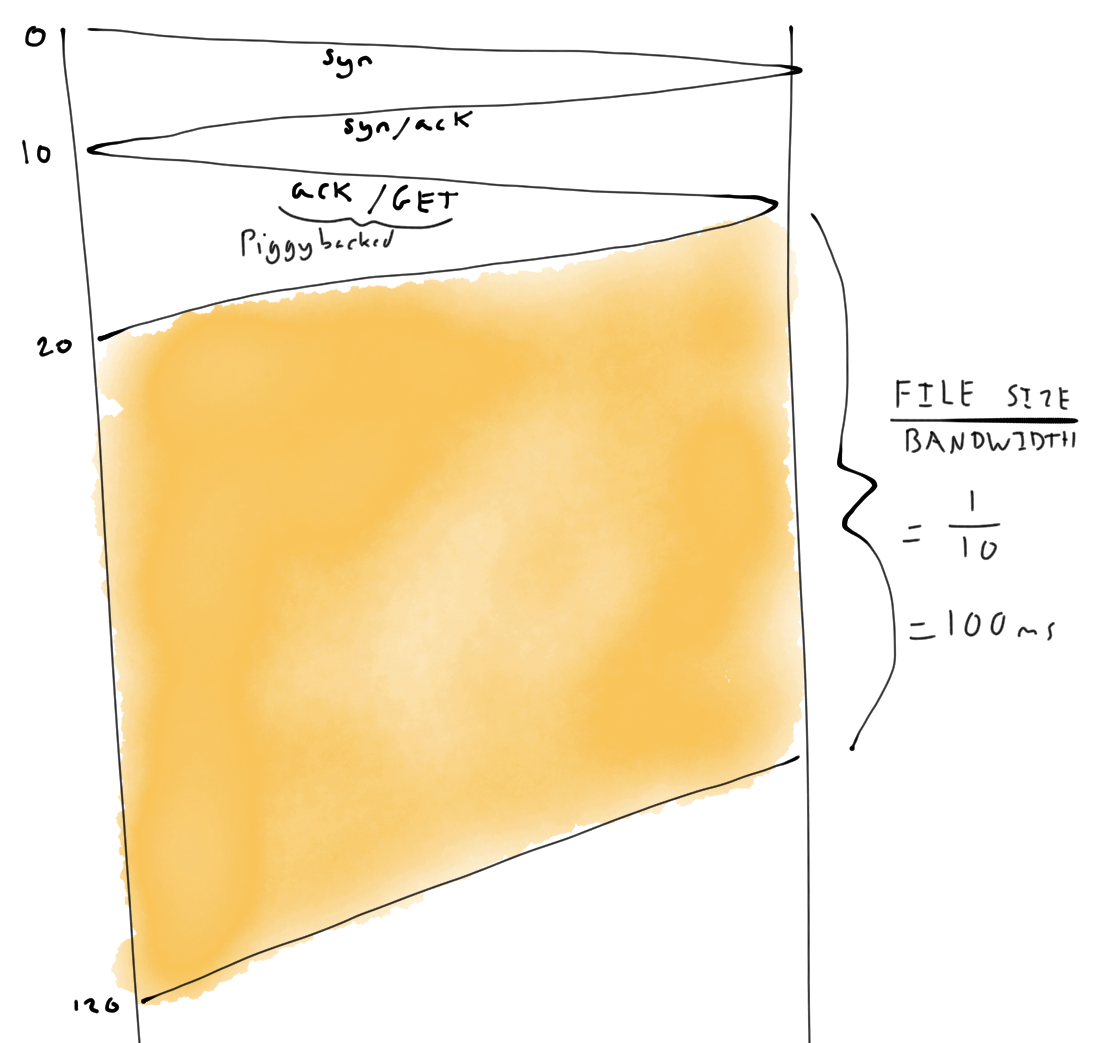
\includegraphics[width=0.8\textwidth]{6-1}
                  \end{center}
                  Since the connection is non persistent the above transmission
                  happens twice (serially) and thus the total time taken is
                  \SI{240}{ms}.
                \end{solution}

              \subsubpart Concurrent requests with non-persistent TCP
                connections?
                \begin{solution}
                  \begin{center}
                    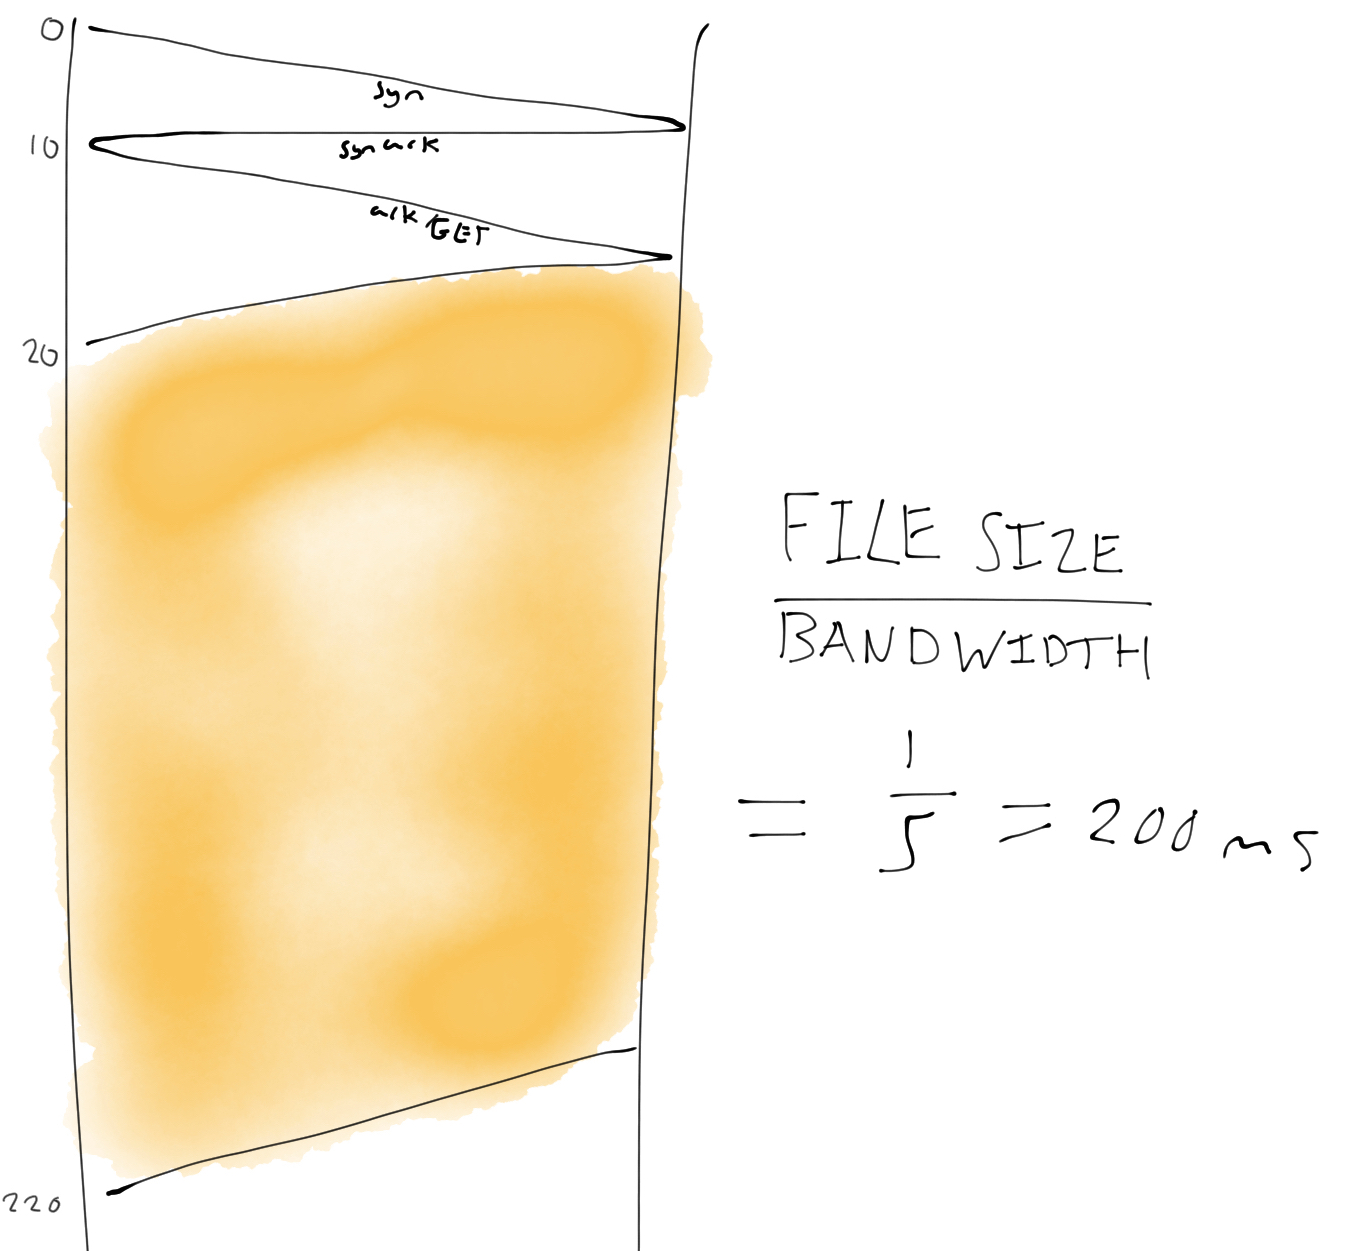
\includegraphics[width=0.8\textwidth]{6-2}
                  \end{center}
                  Since the connections are concurrent only half the bandwidth
                  is available to each one. Total time is \SI{220}{ms}.
                \end{solution}

              \subsubpart Sequential requests within a single persistent TCP
                connection?
                \begin{solution}
                    \begin{center}
                      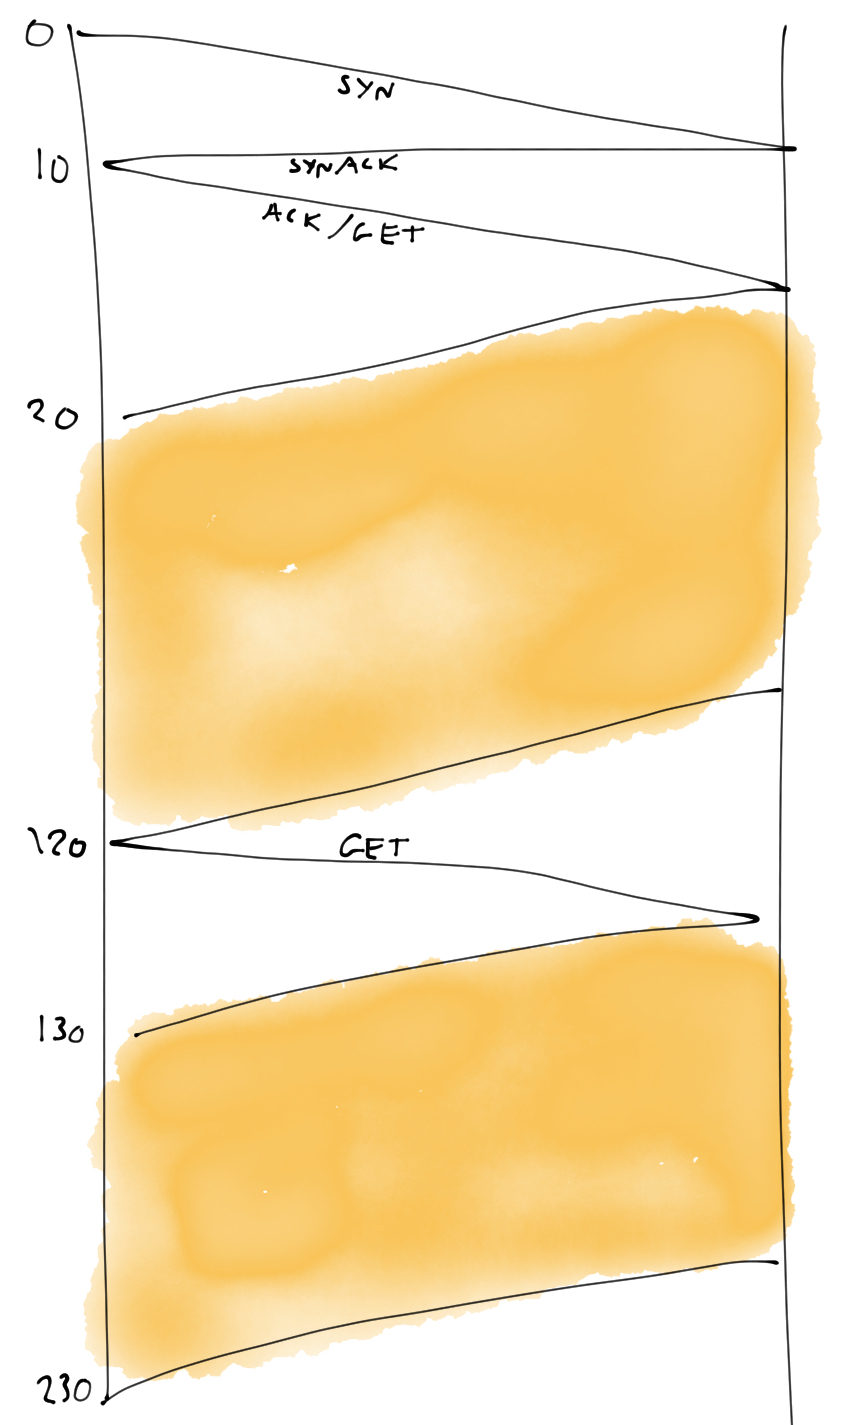
\includegraphics[width=0.5\textwidth]{6-3}
                    \end{center}
                    Total time is \SI{230}{ms}.
                \end{solution}

              \subsubpart Pipelined requests within a single persistent TCP
                connection?
                \begin{solution}
                  \begin{center}
                    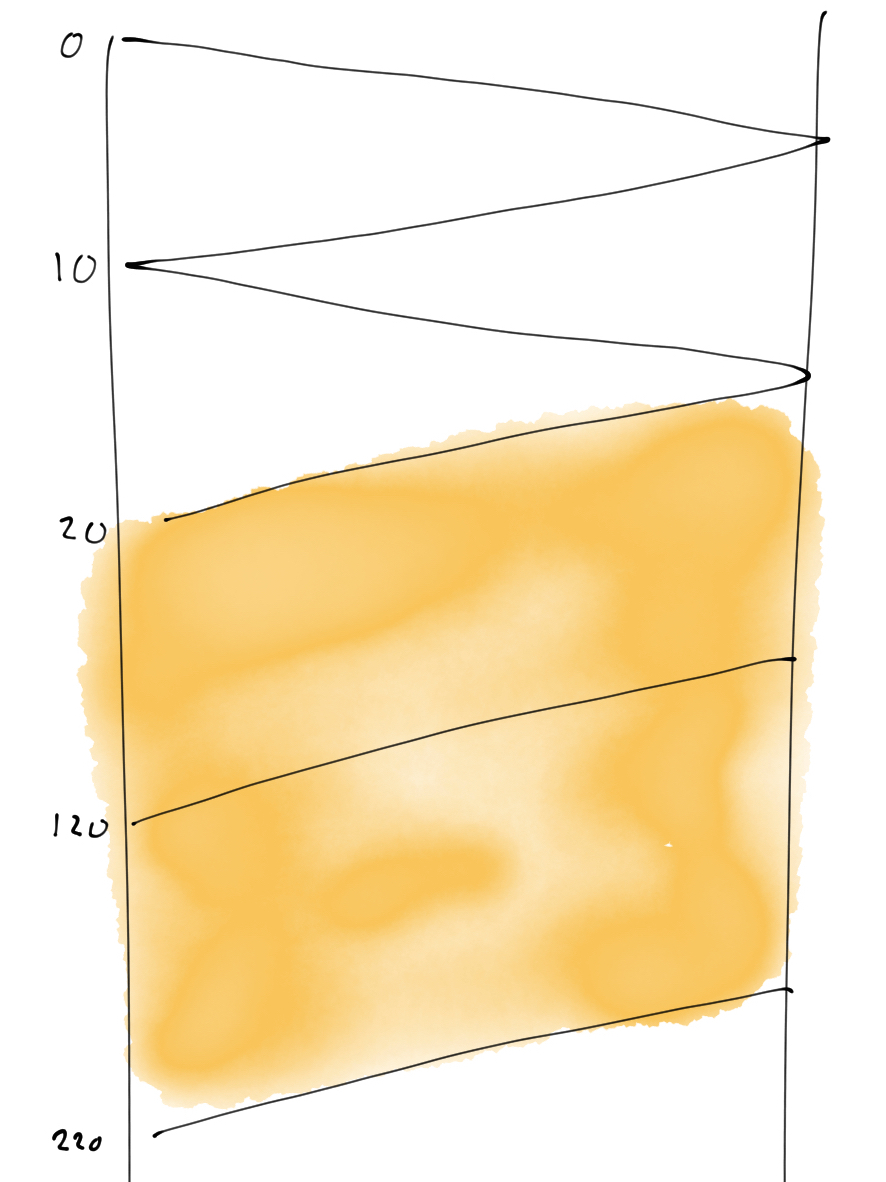
\includegraphics[width=0.5\textwidth]{6-4}
                  \end{center}
                  Total time is \SI{220}{ms}.
                \end{solution}

            \end{subsubparts}
          \subpart Consider the same situation as above, but assume that rather
            than a dedicated link there is a large shared link with many flows
            traversing it, and each TCP connection gets 10Mbps (adding
            additional flows does not significantly change the bandwidth per
            TCP connection, because there are thousands of flows on the link).
            Now, how long does it take $A$ to retrieve both files under the
            following circumstances:
            \begin{subsubparts}
              \subsubpart Sequential (one-at-a-time) requests with
                non-persistent TCP connections?
                \begin{solution}
                  Same as above, \SI{240}{ms}.
                \end{solution}

              \subsubpart Concurrent requests with non-persistent TCP
                connections?
                \begin{solution}
                  \SI{120}{ms} as both requests get \SI{10}{mbps} of bandwidth.
                \end{solution}

              \subsubpart Sequential requests within a single persistent TCP
                connection?
                \begin{solution}
                  Unchanged from previous question, therefore \SI{230}{ms}.
                \end{solution}

              \subsubpart Pipelined requests within a single persistent TCP
                connection?
                \begin{solution}
                  Unchanged from previous question, therefore \SI{220}{ms}.
                \end{solution}

            \end{subsubparts}

          \subpart Consider the first situation, except that $A$ is only
            downloading file $F$ and there is now a cache $C$ between $A$ and
            $B$. All requests from $A$ to $B$ go through cache $C$, and assume
            the bandwidth along the path from $A$ to $C$ is \SI{1}{Gbps} and
            the RTT between $A$ and $C$ is negligible, while the bandwidth
            along the path from $C$ to $B$ is \SI{10}{Mbps} with an RTT of
            \SI{10}{ms}. Note, these are round-trip times, not one way
            latencies. As above, assume that the file is \SI{125}{KB} (i.e.,
            one megabit) and that all TCP SYN/ACK packets and HTTP request
            packets are negligible in size.

            Assume the cache operates as follows: (where the origin server
            refers to the site named in the URL)

            \begin{itemize}
              \item If the object is not in the cache, the request is forwarded
                to the origin server.

              \item If the object is in the cache, and the cache entry has not
                timed out (i.e., the cache TTL has not expired), the object is
                returned to the client.

              \item If the object is in the cache, but the cache entry has
                timed out, the cache issues a conditional-GET to the origin
                server, asking if the object has changed since this object was
                cached: if the origin server responds that it hasn't, the cache
                returns the cached object, otherwise the origin server responds
                with the updated object which the cache forwards to the client.

            \end{itemize}

            How long does it take for $A$ to retrieve the file under the
            following circumstances:

            \begin{subsubparts}
              \subsubpart The file is not in the cache.
                \begin{solution}
                  This depends whether the cache streams the response from the
                  origin server, or stores and forwards it.

                  In the former case it is \SI{120}{ms} as \SI{20}{ms} is
                  required to setup the TCP connection between the cache and the
                  origin server and \SI{100}{ms} to transfer between the origin
                  server and the cache (since we have assumed streaming and the
                  connection between $A$ and $C$ is faster than the connection
                  between $B$ and $C$, the additional time is simply the RTT
                  between $A$ and $C$ which is negligible.).

                  In the latter case it is \SI{121}{ms} since an additional
                  \SI{1}{ms} is required to transfer from $C$ to $A$.
                \end{solution}

              \subsubpart The file is in the cache and the TTL has not expired?
                \begin{solution}
                  \SI{1}{ms} ($\frac{{filesize}}{{bandwidth}}$)
                \end{solution}

              \subsubpart The file is in the cache, the TTL has expired, but
                the file has not been changed.
                \begin{solution}
                  \SI{20}{ms} is required for the SYN/ACK handshake and GET
                  request to the origin server from the cache. Since the file
                  has not been modified the response from the origin server will
                  be negligible in size and the cache then takes a further
                  \SI{1}{ms} transmitting the file back to $A$.

                  Total time = \SI{21}{ms}
                \end{solution}

              \subsubpart The files is in the cache, the TTl has expired and
                the file has changed?
                \begin{solution}
                  This is the same as the file not being in the cache as the
                  overhead of adding an \lstinline|Is-Modified-Since| is
                  negligible. It therefore takes \SI{121}{ms}.
                \end{solution}

            \end{subsubparts}

          \subpart Why is this question answerable \emph{before} you have even
            discussed TCP?
            \begin{solution}
              Well, you need to know about the connection setup part of TCP.
            \end{solution}

        \end{subparts}
    \end{parts}
    \question DNS as an Internet application
    \begin{parts}
      \part Consider the host \lstinline|here.eye.am|, with a local DNS server
        \lstinline|nameserver.eye.am|. \lstinline|here| asks
        \lstinline|nameserver| to resolve the hostname \lstinline|there.you.ar|.
        Assume there are no cached entries relevant to this request and that
        \lstinline|nameserver.eye.am| utilises recursive resolution by default.

        \begin{subparts}
          \subpart Write down the steps taken to resolve
            \lstinline|there.you.ar| and respond to \lstinline|here.eye.am|.
            \begin{solution}
              \emph{This question is a little silly as this is not possible
              over the internet, since the root servers do not support recursive
              DNS queries.}
              \begin{enumerate}
                \item The nameserver makes a recursive request to the root
                  server.
                \item The root server makes a recursive request to the TLD DNS
                  server.
                \item The TLD server makes a recursive request to the
                  authoritative DNS server.
                \item The authoritative DNS server responds to the TLD server.
                \item The TLD server responds to the root server.
                \item The root server responds to the nameserver.
              \end{enumerate}
            \end{solution}

          \subpart Describe the differences between this solution and one
            achieved using an iterative DNS enquiry.
            \begin{solution}
              With iterative DNS queries, every reply goes back to the host and
              it is up to them to then continue the query against the next host.

              This method restricts the advantage of having a cache at the
              resolver since if the query was not in the cache it will not be
              added, as the server will simply refer the client to a different
              server.
            \end{solution}

        \end{subparts}
    \end{parts}
    \SetQuestionNumber{25}
    \question P2P
      \begin{parts}
        \part Peer-to-Peer systems might typically do some combination of three
          tasks, searching (e.g., keyword search), lookup (mapping name to
          location), and download.

          Of the following phrases pick the most appropriate for each question.

          \begin{itemize}
            \item Some form of flooding
            \item Distributed Hash Tables
            \item Chunking
            \item Number of participating peers
            \item Asymmetry of bandwidth
            \item Lack of centralised control
            \item Self-scaling
          \end{itemize}

          \begin{subparts}
            \subpart Which approach is often used for download?
              \begin{solution}
                Chunking
              \end{solution}

            \subpart Which approach is typically used for search?
              \begin{solution}
                Some form of flooding
              \end{solution}

            \subpart Which approach is typically used for lookup?
              \begin{solution}
                Distributed hash tables
              \end{solution}

            \subpart Which factor is most responsible for making chunking
              advantageous?
              \begin{solution}
                Asymmetry of bandwidth
              \end{solution}

          \end{subparts}
        \part Skype and iPlayer both have a P2P heritage. Skype - a P2P
          success, iPlayer less so.
          \begin{subparts}
            \subpart Considering Metcalfe's law, why has Skype been a success?
              \begin{solution}
                Even if products come along that have feature/reliability/cost
                parity (or even better features/reliablility/cost) they will
                find it hard to penetrate the market as ``everyone is on
                skype''.
              \end{solution}

            \subpart Why did iPlayer P2P not succeed whereas iPlayer most
              definitely has succeeded.
              \begin{solution}
                The peer to peer client would upload data even when idle, which
                was not what users were expecting and may have been charged by
                their ISP for. After user backlash and significant investment
                into their streaming infrastructure they moved to HTTP
                downloading.
              \end{solution}

            \subpart Skype is described as a hybrid application - both P2P and
              client-server. Explain this.
              \begin{solution}
                Before Microsoft acquired Skype this statement was accurate
                since it had a central server (actually several server farms)
                that handled authentication, presence, billing etc. Skype calls
                would then be made peer to peer.

                After Microsft acquired Skype its infrastructure has changed
                such that almost all skype calls now go via Skype's network.
              \end{solution}

          \end{subparts}
      \end{parts}
  \end{questions}
\end{document}
